\subsection{ImageNet} \label{sec:ImageNet}
The general purpose model used for transfer learning, is trained on the \texttt{ImageNet}\autocite{imagenet_cvpr09} dataset, consistent of more than 14 million hand annotated images belonging to more than 20.000 categories. For the purpose of this project, a subset of the dataset with 1.000 classes has been chosen.
\begin{figure}[H]
    \centering
    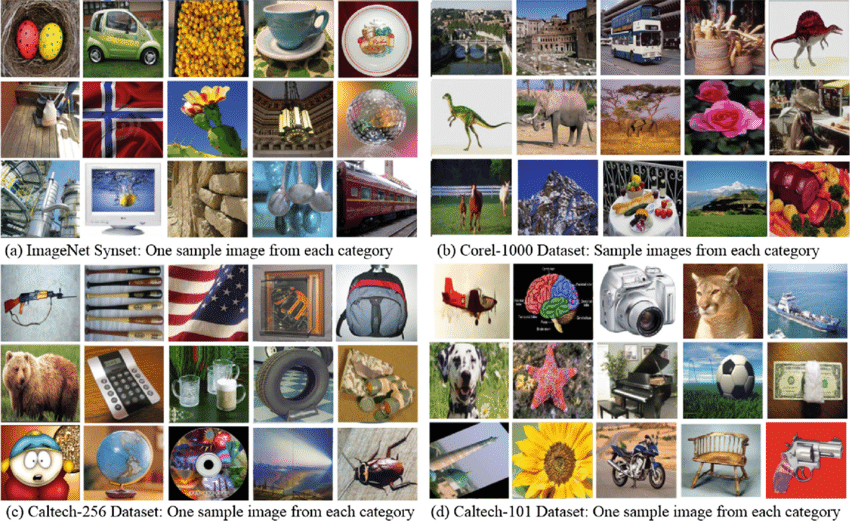
\includegraphics[scale=0.3]{pictures/random/imagenet}
    \caption{Example of ImageNet data. Image source: \autocite{imagenetex}}
    \label{fig:imagenetdata}
\end{figure}
As the pictures show in the above figure, this general purpose model is well trained to detect various different objects.
